\documentclass{article}
\usepackage{soul}
\usepackage{fontenc}
\usepackage[utf8]{inputenc}
\usepackage{amsmath}
\usepackage{amssymb}
\usepackage{pifont}
\usepackage{tikz}
\usepackage{longdivision}
\usepackage{array}
\usepackage{tikz-cd}
\usepackage{amsthm} 





\newcommand{\circled}[1]{\tikz[baseline=(char.base)]{\node[shape=circle,draw,inner sep=2pt] (char) {#1};}}

\usetikzlibrary{shapes.geometric}
\newcommand{\numdiamond}[1]{%
  \tikz[baseline=(char.base)]{
    \node[diamond,draw,inner sep=2pt] (char) {#1};
  }%
}

\begin{document}

\begin{flushleft}
    Page 1 \\
    \vspace*{1em}
\textbf{Naive definition of a set $X$:}\\
\vspace*{0.5em}
\centerline{$X$ = an arbitrary collection of objects.    }
\vspace*{0.5em}
\underline{Problem:} Russell's Paradox:\\
\vspace*{0.5em}
\centerline{$S = \{X \mid X \text{ doesn't contain itself as an element}\}$}
\vspace*{0.5em}
\quad$\circled{1}$ If $S$ is not an element of $S$, then $S$ is an element of $S$\\
\vspace*{0.5em}
\quad$\circled{2}$ If $S$ is an element of $S$, then $S$ is not an element of $S$\\
\vspace*{0.5em}
\quad \underline{Either way}, a contradiction.\\
\vspace*{1em}
The fundamental problem is that a set $X$ must always live in an ambient set $T(X \subseteq T)$. 
But this weakens the naive definition of a set as it implies too much. Therefore, we must add additional axioms known as \underline{Zermelo-Fraenkel Axioms}:
\end{flushleft}

\begin{enumerate}
\item Axiom of Extensionality: if $X$ and $Y$ have the same elements, $X=Y$
\vspace{1em} \\
\centerline {$\forall u (u \in X \equiv u \in Y) \Rightarrow X=Y$ }
\item Axiom of Unordered Pair: For any $a,b$ there exists a set $\{a,b\}$ 
\vspace{1em} \\
\centerline { $\forall a \forall b , \exists c \forall x | (x \in c \equiv (x = a \lor x = b))$ }
\item Axiom of Subsets: $\phi$  \text{ property with parameter} $Y = \{u \in X | \phi (u,p)\}$ 
\item Axiom of Sum set: For any set $X$ there exists a set $Y=0X$ 
\item Axiom of Power set: $Y = P(X)$ set of all sets.
\item Axiom of Infinity 
\item Axiom of Replacement: Image of set under definable function is a set...UNSURE
%UNSURE

\item Axiom of Foundation(Regularity)
\item Axiom of Choice
\end{enumerate}
\newpage
\begin{flushleft}
    Page 2 \\
    Important Operations and Concepts for naive set theory(works in ZFC):
    \begin{align*}
        \begin{array}{@{}l@{\,}l@{}}
        \text{Union:} &\quad X \cup Y = \{z \mid z \in X \text{ or } z \in Y\} \\
        \text{Intersection:} &\quad X \cap Y = \{z \mid z \in X \text{ and } z \in Y\} \\
        \text{Set Difference (complement):} &\quad X \setminus Y = \{z \mid z \in X \text{ and } z \notin Y\} \\
        \text{Cartesian Product:} &\quad X \times Y = \{(x,y) \mid x \in X \text{ and } y \in Y\}
        \end{array}
        \end{align*}
        
        \underline{Additional Ideas}: \\
        
        \begin{align*}
        &\underline{\text{Elemental membership:}} \\
        &a \in X \quad \text{if } a \text{ is an element of } X \\
        &\vspace*{2em} \\
        &\underline{\text{Subset:}} \\
        &X \subseteq Y \quad \text{if every element of } X \text{ is an element of } Y \\
        &\text{Note:} \quad \{a\} \subseteq X \Longleftrightarrow a \in X \\
        &\vspace*{2em} \\
        &\underline{\text{Overset:}} \\
        &\text{When } S \subseteq X \text{ and } S \neq X, \quad \text{we sometimes say that } S \text{ is an } \underline{subset} \text{ of } X \\
        &\text{or that } X \text{ is an } \underline{overset} \text{ of } S. \\
        &\vspace*{2em} \\
        &\underline{\text{Powersets}}: \\
        &\text{Let } X \text{ be a set. The powerset of } X \text{ denotes the set of all subsets of } X. \\
        &\vspace*{1em} \\
        &\text{Example}: \\
        &\begin{aligned}
        X &= \{1,2,3\} \\
        P(X) &= \{\emptyset, \{1\}, \{2\}, \{3\}, \{1,2\}, \{1,3\}, \{2,3\}, \{1,2,3\}\}
        \end{aligned}
        \end{align*}
\end{flushleft}

\newpage

\begin{flushleft}
    Page 3 \\
    \vspace{1em}
    Further additional concepts: 
    \begin{align*}
        \hspace{2em}&\vspace{0em} \\
        \hspace{2em}&\underline{\text{Cardinality}}: \\
        \hspace{2em}&\text{Card}(X) = |X| = (X) \text{ denotes the 'size' of the set } X \text{ which is defined as the} \\
        \hspace{2em}&\text{ordinal number measuring the number of elements of } X. \\
        \hspace{2em}&\vspace{1em} \\
        \hspace{2em}&\underline{\text{Example}}: \\
        \hspace{2em}&\begin{aligned}
        X &= \{ 1,2,3 \} \\
        \text{Card}(\{1,2,3\}) &= 3 \\
        |P(X)| &= 2^{\text{Card}(X)} \text{ (Question: why?)} \\
        |P({1,2,3})| &= 2^3 = 8
        \end{aligned} \\
        \hspace{2em}&\vspace{1em} \\
        \hspace{2em}&\underline{\text{Inductive set or natural numbers}}: \\
        \hspace{2em}&\mathbb{N} = \{1,2,3,4,\ldots,n, n+1, \ldots\} \\
        \hspace{2em}&\text{(Key feature): If } n_1, n_2 \text{ are elements, then } n_1 + 1 \text{ is an element.}
        \end{align*}
    \end{flushleft}


\newpage
\begin{flushleft}
    Page 4 \\
    \vspace{1em}
    \underline{Further concepts}: \\
    \vspace{1em}
    \underline{Relation}: A relation $R$ is a subset of a Cartesian product $X \times Y$. \
    \vspace{1em} \\
    Given two sets $X$ and $Y$, we form the set \
    \vspace{0.5em} \\
    \centerline{ $X \times Y = \{(x,y) \mid x \in X \land y \in Y\}$ } \
    \vspace{0.5em} \\
    \underline{Examples:} \\
    \begin{enumerate}
        \item $\mathbb{R}^{2} = \mathbb{R} \times \mathbb{R} = \{(x,y) \mid x,y \in \mathbb{R}\}$ (INSERT IMAGE) \\
        %UNSURE - insert img
        \item  $\mathbb{R}^{n} := \mathbb{R}^{n-1} \times \mathbb{R} = \mathbb{R}^1\times \ldots \times \mathbb{R}^1$ 
            \vspace{0.5em} \\
            $((x_{1}, \ldots, x_{n-1}), x_{n}) = (x_{1}, \ldots, x_{n-1}, x_{n})$
            \vspace{0.5em} \\
        \item $\{a\} = X, \text{ and } Y \text{ an arbitrary set.}$ 
             \vspace{0.5em} \\
             $X \times Y = \{(a,y) \mid y \in Y\} \neq Y $
             \vspace{0.5em} \\
    
But, $X \times Y \xrightarrow[]{\text{p}} Y, \quad p((a,y)) = y$ (forgets 1st cordinate) is a bijection.\\
Thus, $\{a\} \approx Y$. \\
    
        \item (Bad example) Rational numbers $\mathbb{Q} = \{\frac{p}{q}\mid p,q \in \mathbb{Z}, q \neq 0\}$ \\
            "can be thought as" $\mathbb{Z} \times (\mathbb{Z}^* \{0\}) \quad (p,q) \rightarrow \frac{p}{q}$\\
\end{enumerate}
Actually, to make precise we need the concept of a relation. \\
    \vspace{0.5em} 
\underline{Definition}: We say that a subset $R$ of $X \times Y$ is a relation between $X$ and $Y$. Moreover, we say that $R$
 is a \underline{function} if $(x, y_1), (x, y_2) \in R \implies y_1=y_2$ (CUTOFF)\\
    
\end{flushleft}

\newpage
\begin{flushleft}
    Page 5: \\
    \vspace{1em}
 We will get to functions in a minute, but lets go back to example 4 above: 
 \vspace{0.5em}
\centerline{$S' = \mathbb{Z} \times (\mathbb{Z}^* \setminus {0}) \rightarrow \mathbb{Q}$} \\
\vspace{0.5em}
\centerline{$(p,q) \rightarrow \frac{p}{q}$}
\vspace{1em} 
However, the issue is two fractions can reduce: \\
\vspace{0.5em}
\centerline{ $\frac{p}{q} = \frac{p'}{q'}$ if $pq' = qp'$.} 
\vspace{1em} 
Therefore, let \begin{align*}
    R &\subseteq S \times S \\
    R &= \{ ((p,q),(p',q')) \mid pq'- qp' = 0 \}
    \end{align*}


    
 This is an example of an equivalence relation, often we take $X = Y$ and have relations on $X$ - i.e., Subsets  $R \subseteq X \times X$.
\vspace{1em} \\
\underline{Example 1}: \\
\vspace{0.5em}
$\Delta_X = \{(x,y) \mid x = y\} \text{ is called the diagonal of X.} $\\
\vspace{0.5em}
$\text{This is also an \underline{equivalence relation} and corresponds to the regular notion of}$ \\
$\text{equality } x = x$.


 \vspace{1em} 
   \underline{Example 2}: \\
    \vspace{0.5em}
     $X = \mathbb{N} \{1,2,3,\ldots\} \cup \{0\}$ \\
     $R = \{(x,y) \mid x+y \text{ divisible by } 2\}$   \\            

\end{flushleft}

\newpage
\begin{flushleft}
    Page 6 \\
    \vspace{1em}
    \underline{Example 2 continued}: \\
    \vspace{0.5em}
    Describes an equivalence relation on $\mathbb{W}$ where \\
    \vspace{0.5em}
    $x=y$ iff $x$ and $y$ are even. \quad \underline{or} \quad $x=y$ iff $x$ and $y$ are odd.
    \end{flushleft}
    \begin{center}
    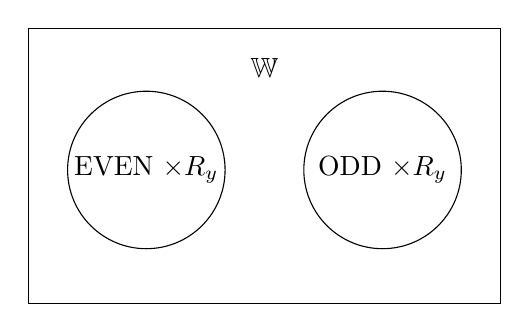
\begin{tikzpicture}
    \node (even) at (0,-0.8) {EVEN $\times R_y$};
    \node (odd) at (3,-0.8) {ODD $\times R_y$ };
    \draw (even) circle (1cm);
    \draw (odd) circle (1cm);
    \node at (1.5,0.5) {$\mathbb{W}$};
    \draw (-1.5,-2.5) rectangle (4.5,1);
    \end{tikzpicture}
    \end{center}
\begin{flushleft}
\underline{Example 3}: \begin{align*}
    R &\subseteq \mathbb{R} \times \mathbb{R}  \\
    R &= \{ (x,y) \mid x < y \}
    \end{align*}
This is a \underline{transitive relation} as $x < y \text{ and } y < z \rightarrow x < z$. \\
\vspace{2em}
\underline{Example 4}: \begin{align*}
    R &\subseteq \mathbb{R} \times \mathbb{R}  \\
    R &= \{ (x,y) \mid x \leq y \}
    \end{align*}
This is both a \underline{transitive} and \underline{ reflexive relation} since $x \leq x$. \\
\end{flushleft}

\newpage
\begin{flushleft}
    Page 7 \\
    \vspace{1em}
    \underline{Example 5}: \\
    \vspace{1em}
    Consider $\mathbb{Z} = \{ \ldots, -2, -1, 0, 1, 2, \ldots \} \quad (\text{ or } \mathbb{W} \text{ or } \mathbb{N})$. \\
    \vspace{0.5em}
    Let $m$ be a natural number $m = 1,2,3,\ldots$ \\
    \vspace{0.5em}
    Then for any $z \in Z$, there exists a unique $q$ called a quotient such that \begin{align*}
    &\boxed{z = mq + r} \quad \text{where} \quad r = 0, 1, 2, \ldots, m-1, \\
    &\frac{z}{m} = q + \frac{r}{m} 
    \end{align*}
    If $m = 2$, then either $z$ is even in which case $z=2q$ or odd and then $z=2q'+1$ \\
    \vspace{0.5em}
    We place an \underline{equivalence relation} on $\mathbb{Z}$ called $\text{mod}_m$ or $\equiv_m$ by
    \begin{align*}
    z &\equiv_m z' \iff z = mq+r \text{ and } z = mq' +r' \\
    z &\equiv z' \mod m \implies r = r'
    \end{align*}
    
\end{flushleft}


\newpage
\begin{flushleft}
    Page 8 \\
    \begin{align*}
    z &\equiv 0 \mod 0 \leftrightarrow \square \\
    z &\equiv 0 \mod 1 \leftrightarrow \text{\textcircled{ }} \\
    z &\equiv 0 \mod 2 \leftrightarrow \diamondsuit \\
    \end{align*}
$\{ \fbox{0},$ $\circled{1}$,$\numdiamond{2}$,$\fbox{3},$ $\circled{4}$,$\numdiamond{5}$,$\fbox{6},$ $\circled{7}$,$\numdiamond{8}$,$\fbox{9},$ $\circled{10}$,$\numdiamond{11}$,$ \ldots,   \} $
\vspace{1em} \\
\underline{Example }: \begin{align*}
    17 &\equiv 7 \pmod{10} \\
    27 &\equiv 7 \pmod{10} \qquad \text{Yet } 17 \not\equiv 27 \mod{3}\\
\end{align*}
$231 \equiv 1111 \mod 4$ ? \underline{To check}: 
\begin{align*}
    &\intlongdivision{231}{4} \quad  \text{r}=\boxed{3}, \text{ so }231 \equiv 3 \mod 4,
    &\intlongdivision{1111}{4} \quad \text{r}=\boxed{3}, \text{ so }  1111 \equiv 3 \mod 4
    \end{align*}

$ \therefore \text{ Yes, } 231 \equiv 1111 \mod 4$\\
\vspace{2em}
\underline{Example} \\
$15 h \equiv 3 \mod 12$ 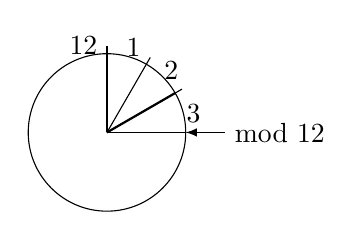
\begin{tikzpicture}
    \draw (0,0) circle (1cm);
    \draw[thick] (0,0) -- (30:1);
    \draw[thick] (0,0) -- (90:1);
    \node[anchor=west] at (1.5,0) {mod 12};
    \draw[-latex] (1.5,0) -- (1,0);
    \draw (0:0cm) -- (0:1cm);
    \node[anchor=0-90] at (0:1.1cm) {3};
    \draw (30:0cm) -- (30:1.1cm);
    \node[anchor=30-90] at (30:1.1cm) {2};
    \draw (60:0cm) -- (60:1.1cm);
    \node[anchor=60-90] at (60:1.1cm) {1};
    \draw (90:0cm) -- (90:1.1cm);
    \node[anchor=90-90] at (90:1.1cm) {12};
    
\end{tikzpicture} \\
    
$ 147 \mod 12 \equiv \text{147 hours after midnight, which is 3 o'clock.}$


\end{flushleft}


\newpage
\begin{flushleft}
    Page 8'
\end{flushleft}

\subsection*{Review: Modular Arithmetic}

On the set $\mathbb{Z} = \{\ldots, -3, -2, -1, 0, 1, 2, 3, \ldots\}$, we place an equivalence relation $\equiv \mod n$ defined by 
\[ x \equiv y \mod n \iff x = mq + r \text{ and } y = mq' + r' \]

$x$ and $y$ are equal provided they have the same remainder.

For each $n$, this relation behaves differently:

\[ 17 \equiv 27 \mod 10 \quad \text{but} \quad 17 \not\equiv 27 \mod 3. \]

\subsection*{Question}
Find all positive integers $x$ such that 
\[ x \equiv 1 \mod 3. \]
\[ \{1, 4, 7, 10, 13, \ldots, 3q + 1, \ldots\} \]

As discussed, arithmetic operations will carry over. What this means is that adding two numbers goes to the right set. 

We define:
\[ a + b := (a + b) \mod n \]
\[ a \cdot b := (a \cdot b) \mod n \]

\subsection*{Example}
\[ (17 + 3) \mod 3 = 20 \mod 3 = 2 \mod 3 \]
(CUTOFF)


\newpage
\begin{flushleft}
    Page 9
\end{flushleft}

When $(x, y)$ is an element of $R$, we write $x R y$ or $x \leq_R y$.

A relation can have a lot of properties. Assume $X = Y$:
\begin{itemize}
    \item \textbf{Reflexive} iff $x \leq_R x$ for all $x \in X$
    \item \textbf{Symmetric} iff $x \leq_R y \implies y \leq_R x$ for all $x, y \in X$
    \item \textbf{Transitive} iff $x \leq_R y$ and $y \leq_R z \implies x \leq_R z$ for all $x, y, z \in X$
\end{itemize}

If $R$ has all of these properties, then it is an \textbf{equivalence relation} on $X$. In this case, we write $= _R$ or just $=$ (Example: $=$ on rational numbers).

More on this topic later.

\textbf{Def:} A function from $X$ to $Y$ is a relation with the following: if for all $x \in X$ and any $y_1, y_2 \in Y$,
\[ x \leq_R y_1 \text{ and } x \leq_R y_2 \implies y_1 = y_2. \]

In this case, we write $y = f(x)$ for $x \leq_R y$.

\newpage
\begin{flushleft}
    Page 10
\end{flushleft}


We say a function $f: X \to Y$ is \textbf{injective} if 
\[ \left[ f(x_1) = f(x_2) \implies x_1 = x_2 \right] \]
\[
    \begin{tikzcd}
        A \arrow[r, hook] & B
        \end{tikzcd}
\]

And we say $f: X \to Y$ is \textbf{surjective} if 
\[ \forall y \in Y, \text{ there exists an } x \text{ such that } f(x) = y \]


\textbf{Provide examples:} 
\[
\begin{array}{l}
X = \mathbb{R} \\
Y = \mathbb{R} \\
R = \text{real numbers}
\end{array}
\]
\[ 
\begin{array}{l}
y = f(x), \quad f(x) = 3x + 1 \quad \text{injective and surjective} \\
y = f(x), \quad f(x) = \sqrt{x} \quad \text{injective but not surjective} \\
y = f(x), \quad f(x) = x^3 - x \quad \text{surjective but not injective}
\end{array}
\]

If a function is both injective and surjective, we say that it is \textbf{bijective} (or a bijection).



\textbf{Thm:} There exists a bijection $f: X \to Y$ if and only if $\text{Card}(X) = \text{Card}(Y)$. 

Question: Are $\mathbb{N}$ and $\mathbb{Q}$ of the same size?


\newpage
\begin{flushleft}
    Page 11
\end{flushleft}
Let $X = Y$ and consider all bijections $f: X \to X$.
This is a set usually denoted
\[
S(X), \quad \text{Sym}(X), \quad \text{Biject}(X), \quad \text{Bi}(X).
\]
This is a prototypical example of a group.

\[
G := \text{Sym}(X)
\]
An element is a bijective map $f: X \to Y$.
\begin{enumerate}
    \item $f \circ g: X \to X$ is bijective. $f(g(x)) = (f \circ g)(x)$ is also bijective.
    \item $(f \circ g) \circ h = f \circ (g \circ h)$.
    \item $1(x) = x$ for all $x$ and $(f \circ 1) = f$, $(1 \circ g) = g$.
    \item If $f: X \to X$ is a bijection, then $f^{-1}: X \to X$ exists and is also a bijection.
\end{enumerate}

These are currently just statements which may be true or not.
We need to prove these statements and the question is, how?

\newpage
\begin{flushleft}
    Page 12
\end{flushleft}
\section*{Cyclic Groups}
Definition for $x$ in $G$:
In general, $x^0 = e$ and $x^n = x \cdot x \cdot \ldots \cdot x$ ($n$ times).

\[
(x^n)^{-1} = (x^{-1})^n
\]

\[
x^{-n} = (x^{-1})^n
\]

\newtheorem*{theorem}{Thm}
\begin{theorem}
    Let $G$ be a group and let $x \in G$. Let $m, n$ be integers. Then:
    \begin{enumerate}
        \item $x^m x^n = x^{m+n}$
        \item $(x^m)^{-1} = x^{-m}$
        \item $(x^m)^n = x^{mn} = (x^n)^m$
    \end{enumerate}
\end{theorem}

\begin{proof}
    For $m$ and $n$ positive, $x^m x^n = x^{m+n}$ (m times $x$).

    If $m, n < 0$, say $m = -r$, $n = -s$ then
    \[
    x^m x^n = x^{-r} x^{-s} = (x^{-1})^r (x^{-1})^s = (x^{-1})^{r+s} = x^{-(r+s)} = x^{m+n}
    \]

    If $m < 0$ (say $m = -r$) and $n > 0$
    \[
    x^m x^n = (x^{-1})^r x^n = (x^{-1})^r x^n = x^{r-n} = x^{m+n}
    \]

    Part (2) and (3) are easy.
\end{proof}



\newtheorem*{definition}{Definition}
\begin{definition}
    Let $x$ be an element of a group $G$. We say $x$ has order $n$ if $x^n = e$ (called finite order).

    If $x$ doesn't have finite order, then we say $x$ has infinite order.
\end{definition}
\newtheorem{example}{Example}
\begin{example}
    \[
    (\mathbb{Z}_3, \oplus) \quad x = [1] \quad [1] + [1] + [1] = [0] \quad \text{order of } [1] = 3
    \]

    What is the order of $[2]$? Of $[0]$?
\end{example}
\newtheorem{example 2}{Example }
\begin{example}
    \[
    (U(\mathbb{Z}_5), \otimes) \quad \text{Calculate the order of all elements}
    \]

    \[
    4^1 \not\equiv 1 \mod 5 \quad 4^2 = 16 \equiv 1 \mod 5 \quad \text{order is } 2
    \]

    \[
    3 \cdot 3 = 9 \equiv 4 \mod 5 \quad 3^2 = 9 \equiv 4 \mod 5
    \]

    \[
    3 \cdot 3 \cdot 3 = 4 \cdot 3 \equiv 12 \equiv 2 \mod 5 \quad \text{order of 3 is 4}
    \]

    \[
    2^4 = 2 \cdot 2 \cdot 2 \cdot 2 \equiv 16 \equiv 1 \mod 5 \quad \text{order of 2 is 4}
    \]
\end{example}





\newpage
\noindent page 13

\textbf{Def.} Let $x$ be an element of a group $G$. We say $x$ has order $n$ if $x^n = e$ (called \textit{finite order}). If $x$ doesn't have finite order, then we say $x$ has \textit{infinite order}.

\textbf{Example:} $(\mathbb{Z}_3, \oplus)$
\[
\begin{aligned}
    x &= [1] \\
    x^2 &= [1] \oplus [1] = [2] \neq [0] \\
    x^3 &= [1] \oplus [1] \oplus [1] = [2] \oplus [1] = [0] = e
\end{aligned}
\]
$[1]$ has order $3$. What is the order of $[2]$? of $[0]$?

\textbf{Example:} $(\mathbb{U}(\mathbb{Z}_5), \otimes)$ Calculate the order of all elements.
\[
\begin{aligned}
    4^1 &\neq 1 \\
    4^2 &= 16 \equiv 1 \pmod{5} \quad \text{(order is 2)} \\
    3 \cdot 3 &= 9 \equiv 4 \pmod{5} \\
    3 \cdot 3 \cdot 3 &= 4 \cdot 3 \equiv 12 \equiv 2 \pmod{5} \\
    3^4 &= 3 \cdot 3 \cdot 3 \cdot 3 = 2 \cdot 3 \equiv 6 \equiv 1 \pmod{5} \quad \text{(order of 3 is 4)}
\end{aligned}
\]

\newpage
\noindent page 14

\textbf{Example:} $G = GL_2(\mathbb{R}) = \left\{ \begin{pmatrix} a & b \\ c & d \end{pmatrix} \mid ad - bc \neq 0 \right\}$

\[
\begin{pmatrix}
    -1 & 0 \\
    0 & -1
\end{pmatrix}^2 = 
\begin{pmatrix}
    1 & 0 \\
    0 & 1
\end{pmatrix}
\]
Thus, this has order 2.

\textbf{Example:} $\mathbb{Z} = \{\ldots, -3, -2, -1, 0, 1, 2, 3, \ldots\}$ Order of 1 is $\infty$.

\textbf{Def.} A group $G$ is called \textit{cyclic} if there is an element $x$ in $G$ such that $G = \{x^n \mid n \in \mathbb{Z}\}$. In this case, $x$ is said to be a \textit{generator} of $G$.

Presentation of a group, compact notation:
In additive notation, $\langle x \rangle = \{nx \mid n \in \mathbb{Z}\}$.

\textbf{Examples:}
\[
\begin{aligned}
    \mathbb{Z} &= \langle 1 \rangle \\
    \mathbb{Z}_n &= \langle 1 \rangle \\
    \mathbb{Z} &= \langle 1 \rangle \text{ (in additive notation)}
\end{aligned}
\]
$\mathbb{Q}$ is not cyclic since $\frac{1}{2} \notin \langle q \rangle$.

\newpage
\noindent page 15

\textbf{Thm} Let $x$ be an element of $G$.
\begin{enumerate}
    \item The order of $x$ is the order of $x^{-1}$.
    \item If the order of $x = n$ and $x^m = e$, then $n$ divides $m$.
    \item If the order of $x = n$ and $\gcd(m, n) = d$, then the order of $x^{m/d} = \frac{n}{d}$.
\end{enumerate}

\textbf{Proof.} Assume $x^n = e$. Write $m = qn + r$. $0 \leq r < n$
\[
\begin{aligned}
    x^m &= e \\
    x^{qn+r} &= e \\
    x^{qn}x^r &= e \\
    (e)^q x^r &= e \\
    x^r &= e \Rightarrow r = 0
\end{aligned}
\]

\newpage
\noindent page 16

\textbf{Thm.} If $G = \langle x \rangle$ and the order of $x = \infty$, then $x^j \neq x^k$ for all $j \neq k$. If the order of $x = n$, then $x^j = x^k$ iff $j \equiv k \pmod{n}$.

\textbf{Def.} Number of elements of $G$ is called the order of $G$.

For finite group with $G = \langle x \rangle$, it must be the case that $G = \{e, x, x^2, x^3, \ldots, x^{n-1}\}$.

\[
\text{Cyclic subgroups}
\]
Let $x$ be an element of order 18. Calculate orders of $x^2, x^3, x^4, x^5, x^{12}$.

\textbf{Exercises:}
\begin{enumerate}
    \item $\mathbb{Z}_{15}$ and list all elements of order 15.
    \item $\mathbb{Z}_{24}$ (cyclic group of order 24). List all elements of order 12.
\end{enumerate}

\newpage
\noindent page 17

Let $X$ be a set (finite or infinite). $S_X = S(X) = \text{Sym}(X) = \{ f : X \to X \mid f \text{ is a bijection} \}$

When $X$ is finite, say $X = \{ 1, 2, 3, \ldots, n \}$, we call $S_n := \text{Sym}(X)$ the \textit{symmetric group of degree} $n$.

\textit{Note:} $|S_n| = n!$

For $f \in S_X$, $f$ \textit{shuffles the elements} $\{ 1, 2, 3, \ldots, n \}$. Therefore we can represent $f$ explicitly by writing:
\[
\begin{pmatrix}
1 & 2 & 3 & \cdots & n \\
f(1) & f(2) & f(3) & \cdots & f(n)
\end{pmatrix}
\]

For example, consider:
\[
\begin{pmatrix}
1 & 2 & 3 & 4 \\
2 & 4 & 1 & 3
\end{pmatrix}
\begin{pmatrix}
1 & 2 & 3 & 4 \\
3 & 2 & 4 & 1
\end{pmatrix}
\]

$h = f \circ g$ Find where each element goes.

\newpage
\noindent page 18

Let $X_1, X_2, \ldots, X_r$ $(1 \leq r \leq n)$ be $r$ distinct elements of $\{ 1, 2, \ldots, n \}$. The $r$-cycle $(X_1, X_2, \ldots, X_r)$ is the element of $S_n$ such that
\[
\begin{aligned}
    X_1 &\to X_2 \\
    X_2 &\to X_3 \\
    &\vdots \\
    X_{r-1} &\to X_r \\
    X_r &\to X_1
\end{aligned}
\]

For example,
\[
\begin{pmatrix}
1 & 2 & 3 & 4 \\
1 & 4 & 3 & 2
\end{pmatrix} = (2, 4)
\]
The identity permutation can be written as $(1)(2)(3)(4)$.

Two cycles are disjoint if their elements as a set are disjoint: $\{ x_1, \ldots, x_r \} \cap \{ y_1, \ldots, y_s \} = \emptyset$.

\textbf{Theorem:} For any $f$ in $S_n$, there exist disjoint cycles $\sigma_1, \sigma_2, \ldots, \sigma_m$ such that $f = \sigma_1 \circ \sigma_2 \circ \ldots \circ \sigma_m$.

\newpage
\noindent page 19

\textbf{Proof.} Choose some $x_1 \in \{ 1, \ldots, n \}$. 
\[
\begin{aligned}
    x_2 &= f(x_1) \\
    x_3 &= f(x_2) \\
    &\vdots
\end{aligned}
\]

There must be a \textit{first element} $x_k$ which is the same as a previous element $x_j \to$ say $x_k = x_j$. $j < k$. In this case $j = 1$ since $x_k = x_j$ implies $x_k = x_{j-1}$ which contradicts the minimality of $k$ because $f$ is one-to-one.

Thus, the first $k-1$ elements $x_1, x_2, \ldots, x_{k-1}$ are distinct with $x_k = x_1$. Thus $f = f_1 \circ h_1$ with $f_1 = (x_1, x_2, \ldots, x_{k-1})$ with $h_1$ permutes elements other than those above.

We can continue this argument until
\[
\begin{aligned}
    f &= f_1 \circ f_2 \circ h_2 \\
    f &= f_1 \circ f_2 \circ f_3 \circ h_3 \\
    &\vdots \\
    f &= f_1 \circ f_2 \circ f_3 \circ \ldots \circ f_m \circ h_m \quad \text{where } h_m \text{ has nothing left to permute.}
\end{aligned}
\]
\newpage
\noindent page 20

\[
\begin{pmatrix}
1 & 2 & 3 & 4 & 5 & 6 & 7 & 8 \\
3 & 5 & 7 & 4 & 2 & 8 & 1 & 6
\end{pmatrix}
= (1 \ 3 \ 7) \circ 
\begin{pmatrix}
1 & 2 & 3 & 4 & 5 & 6 & 7 & 8 \\
1 & 5 & 3 & 4 & 2 & 6 & 7 & 8
\end{pmatrix}
\]
\[
= (1 \ 3 \ 7) \circ (2 \ 5)
\]
\[
= (1 \ 3 \ 7) \circ (2 \ 5) \circ (6 \ 8)
\]

This is similar to factorization of integers into primes.

\textit{Note that disjoint cycles commute.}

\textbf{Theorem:} For $n \geq 2$, any permutation in $S_n$ factors as a product of transpositions $(a \ b)$.

\textbf{Proof:}
\[
(1) = (1 \ 2) \circ (2 \ 1)
\]
For a general $r$-cycle with $r \geq 2$,
\[
(x_1 \ x_2 \ \ldots \ x_r) = (x_1 \ x_r) \circ (x_1 \ x_{r-1}) \circ \ldots \circ (x_1 \ x_2)
\]

\textbf{Example:}
\[
\begin{pmatrix}
1 & 2 & 3 & 4 & 5 & 6 & 7 & 8 \\
3 & 5 & 7 & 4 & 2 & 8 & 1 & 6
\end{pmatrix}
= (1 \ 3 \ 7) \circ (2 \ 5) \circ (6 \ 8)
\]
\[
= (1 \ 7) \circ (1 \ 3) \circ (2 \ 5) \circ (6 \ 8)
\]

\textbf{Def.} A permutation is \textit{even} if it can be written as an even number of transpositions and \textit{odd} if it can be written as an odd number of transpositions.

\newpage
\noindent page 21

\textbf{Theorem:} No permutation is both even and odd. Why? 

$A_n = \{ f \in S_n \mid f \text{ is even} \}$ for $n \geq 2$.

\textbf{Theorem:} $A_n$ is a subgroup of $S_n$ and $|A_n| = \frac{n!}{2}$. Why? 

Investigate $S_3$:
\[
f = (1 \ 2 \ 3), \quad g = (1 \ 3 \ 2)
\]
\[
S_3 = \{ e, f, f^2, g, fg, f^2g \} = D_3
\]

\newpage
\noindent page 22

\textit{Review Exam. Quiz 6.}

\textbf{Computations with $A_3$}

\[
|A_3| = \frac{3!}{2} = 3
\]
\[
A_3 = \{ (1), (1 \ 3 \ 2), (1 \ 2 \ 3) \} = (1 \ 2 \ 3)
\]

\textbf{Claim:} $A_3$ is normal in $S_3$.

\textbf{Def.} We say a subgroup $N < G$ is \textit{normal} (written $N \triangleleft G$) if $gN = Ng$ for all $g$ in $G$.

Note: 
\[
gN = \{ g \cdot x \mid x \in N \}
\]
\[
Ng = \{ x \cdot g \mid x \in N \}
\]

When $N \triangleleft G$, then the left cosets are equal to right cosets.

\textit{Remark:} In general, $H < G$ general subgroup
\[
|H| \cdot [G : H] = |G| \quad \text{equal to the number of left cosets}
\]
\newpage
\noindent page 23

We know $S_n \overset{\sigma}{\to} \{-1, 1\}$ where $\sigma(\varphi) = (-1)^{\text{sign of } \varphi}$ is a group homomorphism and $\ker(\sigma) = A_n$, which provides an automatic proof of normality.

\textit{Let's check directly:}
\[
\begin{aligned}
    (12)(132)(12)^{-1} &= (12)(132)(12) \\
    (12)(123)(12)^{-1} &= (12)(123)(12) \\
    (13)(132)(13)^{-1} &= (13)(132)(13) \\
    (23)(132)(23)^{-1} &= (23)(123)(23)
\end{aligned}
\]

\textbf{Groups up to order 16:}
\[
\begin{array}{ll}
1 & \text{trivial group} \\
2 & \mathbb{Z}/2\mathbb{Z} \\
3 & \mathbb{Z}/3\mathbb{Z}, \ A_3 \\
4 & \mathbb{Z}/4\mathbb{Z} \text{ and } K = \mathbb{Z}/2\mathbb{Z} \times \mathbb{Z}/2\mathbb{Z} \\
5 & \mathbb{Z}/5\mathbb{Z} \\
6 & \mathbb{Z}/6\mathbb{Z} \text{ non-abelian, } D_3 \\
7 & \mathbb{Z}/7\mathbb{Z} \\
8 & \mathbb{Z}/8\mathbb{Z}, \ \mathbb{Z}/4\mathbb{Z} \times \mathbb{Z}/2\mathbb{Z}, \ \mathbb{Z}/2\mathbb{Z} \times \mathbb{Z}/2\mathbb{Z} \times \mathbb{Z}/2\mathbb{Z}, \ \text{non-abelian,} \ D_4 \\
9 & \mathbb{Z}/9\mathbb{Z} \\
10 & \mathbb{Z}/10\mathbb{Z}, \ \text{non-abelian} \ D_5 \\
12 & \mathbb{Z}/12\mathbb{Z}, \ \text{abelian}, \ D_6 \\
16 & \mathbb{Z}/16\mathbb{Z}, \ \mathbb{Z}/8\mathbb{Z} \times \mathbb{Z}/2\mathbb{Z}, \ \mathbb{Z}/4\mathbb{Z} \times \mathbb{Z}/4\mathbb{Z}, \ \mathbb{Z}/4\mathbb{Z} \times \mathbb{Z}/2\mathbb{Z} \times \mathbb{Z}/2\mathbb{Z}, \ \mathbb{Z}/2\mathbb{Z} \times \mathbb{Z}/2\mathbb{Z} \times \mathbb{Z}/2\mathbb{Z} \times \mathbb{Z}/2\mathbb{Z}
\end{array}
\]

\newpage
\noindent page 24

$A_4 = \langle a, b \rangle$ where $a = (12)(34)$ and $b = (123)$.

$A_4$ does not have a subgroup of order 6 as its index would be 2.

\textbf{Proof:} Any subgroup of index 2 must contain all elements of odd order.

Let $H$ be finite, $H \triangleleft G$.
\[
|G : H| = 2
\]

\textit{Note that index 2 implies normality.}

Let $g$ be any element of $G$. If $g \notin H$, then $gH \neq Hg$. If $g \in H$, cosets are $H$ and $gH$. Since left cosets are disjoint, $gH = G - H$. But right cosets are also disjoint, $Hg = G - H$. Thus, $H$ is normal.

Thus, if $H \triangleleft A_4$, consider coset $\{3$-cycle$\}$ $H$ and cosets $H, xH, x^2H$. $A_4$ implies $x^2H = gH$ since if $x \cdot H = H \Rightarrow x^{-1} \cdot e \in H \Rightarrow x \cdot H = H$ or $x \cdot H = x^2H \Rightarrow x = e$. 

\newpage
\noindent page 25

Next: Applications, solvable groups, and extra groups by page 30 of supplementary text after mid Isomorphism Theorems.

\textbf{Cayley's Theorem:} Every group $G$ can be identified with a subgroup of $\text{Sym}(G)$.

\textbf{Proof:} This is established by left group action $G \times G \to G$.

In general, a group homomorphism
\[
\varphi: G \to \text{Sym}(X) \text{ is equivalent to a group action } G \times X \to X.
\]
1. When $\ker(\varphi) = \{ e \}$, the group action is called \textit{faithful}.
2. When $\varphi$ is surjective, we say the group action is \textit{transitive}.

\textbf{Theorem:} $G \times X$ and $\left|G\right| / \left|X\right| \Rightarrow \ker(\varphi) = \{ e \}$, the action is not faithful.

\newpage
\noindent page 26

\textbf{The Orbit-Stabilizer Theorem:} $G \times X \to G \times X$ finite.

For any $x \in X$, $|G : G_x| = \#(G / G_x)$.

\textbf{Proof:} Consider the mapping $\varphi: G / G_x \to O_x$, given by $\varphi(h G_x) = h \cdot x$.
1. $\varphi$ is well-defined: $g G_x = h G_x \Rightarrow h^{-1}g \in G_x$ and so $\varphi(h^{-1}g \cdot x) = \varphi(h \cdot x)$.
2. $\varphi$ is surjective: $\varphi(g G_x) = \varphi(h G_x)$ same element of orbit.
3. $\varphi$ is injective: $\varphi(g G_x) = \varphi(h G_x) \Rightarrow \varphi(h \cdot x) = \varphi(g \cdot x)$.

\textbf{Corollary:} $|G : G_x| = \# O_x$ since $O_x = |G : G_x|$ for all $x \Rightarrow G \times X \to X$ transitive.
\newpage
\noindent page 27

As we saw before, the conjugation action $\varphi: G \to \text{Sym}(G)$ has $\ker(\varphi) = Z(G)$, the center of $G$.

\textit{Proof demonstrated last class.}

\textbf{Burnside's Orbit Counting Theorem:}
Let $G$ be a finite group,
\[
\frac{1}{|G|} \sum_{g \in G} | \text{Stab}_G(g) | = \text{number of orbits of } G \text{ on } X
\]
In the case that the group action is conjugation,
\[
\frac{1}{|G|} \sum_{g \in G} | C_G(g) | = \text{number of conjugacy classes in } G
\]
where $C_G(g) = \{ h \in G \mid hg = gh \}$, the number of elements that commute with $g$.

\newpage
\noindent page 28

Thus, for $h \in G$, the orbit of the conjugation action is given by
\[
O_h = \{ ghg^{-1} \mid g \in G \} = [h] \text{ (conjugacy class of } h \text{)}
\]
The stabilizer subgroup of $h$ is the centralizer of $h$ in $G$,
\[
\text{Stab}(h) = \{ g \in G \mid ghg^{-1} = h \} = C_G(h)
\]
and
\[
|O_h| = |[h]| = [G : C_G(h)] \quad \text{(number of cosets)}
\]

Because $X = G$ for the conjugation action, we can write
\[
|G| = |O_{g_1}| + |O_{g_2}| + \ldots + |O_{g_m}| \text{ for some } g_1, g_2, \ldots, g_m
\]
Note $|O_h| = 1$ iff $h \in Z(G)$ (center).

\textbf{The Class Equation:}
\[
|G| = |Z(G)| + \sum_{i} [G : C_G(y_i)]
\]
This equation reveals the deeper structure of the group.

\newpage
\noindent page 29

\textbf{Def.} A $p$-group $P$ is any group of order $|P| = p^n$ with $p$ a prime.

\textbf{Lemma:} Let $P$ be a $p$-group acting on a set $X$. If $|X|$ is not divisible by $p$, then there is at least one fixed element in $X$.

\textbf{Proof:} Generally, $|X| = |O_{x_1}| + \ldots + |O_{x_n}|$.

Since $P$ is a $p$-group, $|O_{x_i}|$ is a power of $p$.
Thus, $|O_{x_i}| = 1$ for some $i$.
Otherwise, if $|O_{x_i}| > 1$ for all $i$, $p$ divides $|X|$, a contradiction.

But if $|O_{x_i}| = 1$, then $O_{x_i} = \{x_i\}$.

\newpage
\noindent page 30

\textbf{Proposition:} For a prime $p$ and a $p$-group $P$, the center of $P$ is not the trivial subgroup.

\textbf{Proof:} If $Z(P) = \{e\}$ and the class equation implies that the other conjugacy classes $[y_i]$ have cardinality $p^k$ for some $k \geq 1$,
\[
|P| = p^n = 1 + p^m \quad \text{which is impossible}
\]
\textbf{Corollary:} For a prime $p$, a group of order $p^2$ is abelian.

\textbf{Proof:} We know by the previous lemma $|Z(P)| = p \text{ or } p^2$.
If $|Z(P)| = p^2$, then $Z(P) = P$, so $P$ is abelian.
Suppose $|Z(P)| = p$ and $x \in P$ and $x \notin Z(P)$.
The centralizer of $x$,
\[
C_P(x) = \{ g \in P \mid gx = xg \} \supseteq Z(P)
\]
Thus, $Z(P) \subset C_P(x) \subset P$, but then $|C_P(x)| \neq p^2$, and $C_P(x) = P$.
Thus, $x$ commutes with every element of $P$, and so $x \in Z(P)$, a contradiction.

\newpage
\noindent page 31

\textbf{Cauchy's Theorem:} For a finite group $G$, if $p$ is a prime that divides $|G|$, then there is an element $g \in G$ of order $p$.

Ludwig Sylow extended the above result.

\textbf{Def.} Let $p$ be a prime number and let $G$ be a finite group. Suppose $|G| = p^em$ where $p \nmid m$. A \textit{Sylow $p$-subgroup} of $G$ is a subgroup $P$ that is a $p$-group of order $p^e$.

\textbf{The Sylow Theorems:} Suppose $p$ is a prime and $G$ is a finite group for which $p$ divides $|G|$. Then:
\begin{enumerate}
    \item $G$ contains a Sylow $p$-subgroup.
    \item The Sylow $p$-subgroups of $G$ are conjugates of one another.
    \item If $P$ and $Q$ are Sylow $p$-subgroups of $G$, then $\exists x \in G$ such that $P = xQx^{-1}$.
    \item If $|G| = p^em$ and $n_p$ denotes the number of Sylow $p$-subgroups of $G$, then $n_p$ divides $m$ and $n_p \equiv 1 \pmod{p}$.
\end{enumerate}

\newpage
\noindent page 32

\textbf{Proposition:} If $|G| = p^km$, $p \nmid m$, then $G$ is not a simple group.

For example,
\[
\begin{aligned}
    30 &= 2 \cdot 3 \cdot 5, \\
    56 &= 2^3 \cdot 7, \\
    60 &= 2^2 \cdot 3 \cdot 5, \\
    63 &= 3^2 \cdot 7, \\
    72 &= 2^3 \cdot 3^2, \\
    90 &= 2 \cdot 3^2 \cdot 5, \\
    105 &= 3 \cdot 5 \cdot 7, \\
    108 &= 2^2 \cdot 3^3, \\
    120 &= 2^3 \cdot 3 \cdot 5.
\end{aligned}
\]

None of these orders can form simple groups, as they all have non-trivial Sylow $p$-subgroups.

\newpage
\noindent page 33

A brief note:
\[
PSL_2(\mathbb{F}_7) = PSL_2(7)
\]
is a simple group of order 168. This explains why 168 was stubborn.

This is an example of a matrix group over a finite field. As we will see later, $\mathbb{Z}/n\mathbb{Z}$ is actually a ring, but when $n = p^e$ with $p$ a prime, it is actually a field.

Thus, we can talk about vector spaces $V$ over a field and in particular over $\mathbb{Z}/p\mathbb{Z}$.

\textit{Note:}
\[
\begin{aligned}
    GL_n(k) &= \{ n \times n \text{ matrices with entries in } k \text{ with } \det(A) \neq 0 \}, \\
    SL_n(k) &= \{ A \in GL_n(k) \mid \det(A) = 1 \}, \\
    PGL_n(k) &= GL_n(k) / Z(GL_n), \\
    PSL_n(k) &= SL_n(k) / Z(SL_n).
\end{aligned}
\]
The center of the group is identified with the $n$-th roots of unity in $k$.

\textbf{Theorem:} $PGL_n(k) \cong PSL_n(k)$ iff every element of $k$ has an $n$-th root in $k$.

For example, $PGL_n(\mathbb{C}) \cong PSL_n(\mathbb{C})$ but $PGL_n(\mathbb{R}) > PSL_n(\mathbb{R})$.

\newpage
\noindent page 34

This can be defined over a ring $R$ with the most important example being the modular group $\Gamma = PSL_2(\mathbb{Z})$, linear fractional transformations of upper half-plane.

This group is actually generated by two elements:
\[
S: z \mapsto -\frac{1}{z} \text{ (reflection)}, \quad T: z \mapsto z+1 \text{ (translation)}.
\]

In the 1830's, after finding the alternating group $A_n$, Galois discovered another family of simple groups as $PSL_2(q)$ where $q$ is a power of a prime.

We have the so-called exceptional isomorphisms:
\[
\begin{aligned}
    PSL_2(2) &\cong S_3, \\
    PSL_2(3) &\cong A_4, \\
    PGL_2(3) &\cong S_4.
\end{aligned}
\]
Also,
\[
\begin{aligned}
    PSL_2(4) &\cong A_5, \\
    PSL_2(5) &\cong A_5, \\
    PSL_2(9) &\cong A_6 \quad \text{unless } (n, q) = (2, 2) \text{ or } (2, 3).
\end{aligned}
\]

Finally,
\[
PSL_2(7) \cong PSL_3(2) \text{ (second smallest non-abelian simple group)}.
\]

There are a few other exceptional isomorphisms.

\newpage
\noindent page 35

\textbf{Question:} Why does $PSL_2(7)$ have 168 elements?

Let
\[
A = \begin{pmatrix}
a & b \\
c & d
\end{pmatrix}
\]
Total possibilities for the first column is $7^2 - 1 = 49 - 1 = 48$.

Then we must solve the equation $ad - bc = 1$. $ay - bx \neq 0$.

Continue to count: Column 2 must not be a multiple of Column 1. So we have 49 - 1 possibilities like before, except we have to account for:
\[
\begin{pmatrix}
1 & 0 \\
0 & 1
\end{pmatrix},
\begin{pmatrix}
2 & 0 \\
0 & 1
\end{pmatrix},
\ldots,
\begin{pmatrix}
6 & 0 \\
0 & 1
\end{pmatrix}.
\]
So, 49 - 7 possibilities for column 2 = 42.

Now $\det(A) = 1, 2, 3, 4, 5, 6 = 7!$. We must divide by 6 to reduce down to $SL_2(7)$. Thus, $|PSL_2(7)| = 48 \cdot 42 / 7 \cdot 24 / 7 = 168$.

\textit{On another note:} $3^{\text{rd}} \quad \frac{\left| S_5 \right|}{|A_5|} = 5$. Thus, $S_n / A_n \cong S / S_5 N$.

\textbf{Related to Quiz 11:}
\[
PGL_2(\mathbb{C}) = GL_2(\mathbb{C}) / (\mathbb{Z}_2 \times N) = PSL_2(\mathbb{C}) \cong SL_2(\mathbb{C}) / E.
\]
\newpage
\noindent page 36

\textbf{Notes on Rings:}

There are slightly different definitions of rings. For us, the general idea is that a ring is a set $R$ with two operations $(R, +, \cdot)$ where $(R, +)$ is an abelian group with additive identity $0$.

Then $(R, \cdot)$ can either be one of the three:
\begin{enumerate}
    \item Semigroup
    \item Monoid
    \item Commutative Monoid
\end{enumerate}

Since I like commutative algebra, I choose option B and then later specialize to option C. In general, we mainly focus on option C.

Therefore, a ring is a set $R$ with set theoretic maps $+: R \times R \to R$ and $\cdot: R \times R \to R$ which satisfy:
\begin{enumerate}
    \item $\forall a, b, c \in R, a + (b + c) = (a + b) + c$ \quad (associativity)
    \item $\forall a, b \in R, a + b = b + a$ \quad (commutativity)
    \item $\exists 0 \in R \text{ such that } a + 0 = a$ \quad (additive identity)
    \item $\forall a \in R, \exists -a \in R \text{ such that } a + (-a) = 0$ \quad (additive inverse)
    \item $\forall a, b, c \in R, a \cdot (b \cdot c) = (a \cdot b) \cdot c$ \quad (associativity of multiplication)
    \item $\forall a, b, c \in R, a \cdot (b + c) = a \cdot b + a \cdot c$ \quad (left distributivity)
    \item $\forall a, b, c \in R, (a + b) \cdot c = a \cdot c + b \cdot c$ \quad (right distributivity)
\end{enumerate}

\newpage
\noindent page 37

If, in addition, we have property 9
\[
\forall a, b \in R, a \cdot b = b \cdot a
\]
then we say that $R$ is a commutative ring. When the context is clear, $CR \equiv \text{Commutative Ring} = \text{Ring}$.

If, in addition, we have property 10 (inverses), then we say $R$ is a field.
\[
\forall a \in R \setminus \{ 0 \}, \exists b \in R \text{ such that } a \cdot b = b \cdot a = 1
\]

\textit{An aside:}

If we have property 10 but not property 9, then we say that $R$ is a skew-field or a division ring.

We can use other notations such as a semi-ring (basically $(R, +)$ semigroup and $(R, \cdot)$ semigroup with 0 additive identity).

\newpage
\noindent page 38

\textbf{Next: Ring homomorphism, subrings, ideals, isomorphism theorem.}

\textbf{Examples:}
\begin{enumerate}
    \item Prototypical example $(\mathbb{Z}, +, \cdot)$
    \item Another great example $(\mathbb{Z}/n\mathbb{Z}, +, \cdot)$
    \item When $n = p$ a prime, a field (finite field) $(\mathbb{Z}/p\mathbb{Z}, +, \cdot)$ is usually denoted $\mathbb{F}_p$.
    \item Non-commutative example: $M_n(\mathbb{R}) = n \times n$ matrices with matrix addition and matrix multiplication.
\end{enumerate}

\textbf{Endomorphism of a Group:}
$G \to R$

For these, go into non-commutative stuff.

\newpage
\noindent page 39

In general, given a group $G$, there is a such thing as a group ring:
\[
R[G] = \{ f: G \to R \mid f \text{ finite support} \}
\]
Thus, an element can be written as:
\[
f = \sum_{g \in G} f(g)g \quad \text{(example of free construction)}
\]

If you take an abelian group, you get commutative rings (example polynomial rings). Otherwise, you get non-commutative rings.

\[
R[\mathbb{Q}] \quad \text{elements are } x^2 + x(g) + \ldots
\]

These are the so-called quaternions over $\mathbb{R}$, or otherwise the so-called ring of differential operators.

\textit{Note:} Actually for a monoid $M$, we can form $R[M]$.

\newpage
\noindent page 40

\textbf{Free Groups:}

Given a set $S$, we define $F_S$ the free group generated over $S$ by all finitely supported maps $f: \mathbb{Z} \to S$.

\[
\sum f(x) e_x \quad \text{(finite support)}
\]

Addition notation because it is abelian. A similar construction can occur if we want a non-commutative group.

\[
\langle S \rangle = \{ x_1^{a_1} x_2^{a_2} \ldots x_n^{a_n} \mid x_i \in S, a_i \in \mathbb{Z} \setminus \{ 1 \} \}
\]

with identification
\[
x_i^m x_i^n = x_i^{m+n}, \quad x_i^{-m} x_i^m = 1 \quad \text{(identity)}
\]

\textit{Universal Properties:}
\[
F_S \to G \quad \text{abelian}
\]

For general free group:
\[
S \to \langle S \rangle \to G
\]
\newpage
\noindent page 41

\textbf{Further examples of rings:}
1. $R[x]$: polynomial ring over $R$, $R$ ring.
\[
R[x] = \{ a_n x^n + \ldots + a_0 \mid a_i \in R \}
\]
\[
p(x) = a_n x^n + a_{n-1} x^{n-1} + \ldots + a_0
\]
\[
q(x) = b_m x^m + b_{m-1} x^{m-1} + \ldots + b_0
\]
\[
p(x) \cdot q(x) = \sum a_i b_j x^{i+j}
\]
Generally speaking, polynomial rings have additional properties (ID, UFD, PID).

2. $R[x_1, \ldots, x_n]$: multivariate polynomial ring over $R$.

In general, given a polynomial $p(x_1, \ldots, x_n) \in S[x_1, \ldots, x_n]$ and $s_1, \ldots, s_n \in R$:
\[
\text{evaluation} \quad p(x_1, \ldots, x_n) \mapsto p(s_1, \ldots, s_n)
\]
This is a ring homomorphism.

\newpage
\noindent page 42

Let $S$ and $R$ be two rings. We say that $f: S \to R$ is a ring homomorphism if:
\begin{enumerate}
    \item $\forall x, y \in S, \quad f(x + y) = f(x) + f(y)$
    \item $\forall x, y \in S, \quad f(x \cdot y) = f(x) \cdot f(y)$
    \item $f(1_S) = 1_R$
\end{enumerate}
Condition 3 is necessary if option A definition is allowed.

\textbf{Some basic examples:}
\begin{enumerate}
    \item $R \to R[x]$, $R$ is a subring of $R[x]$.
    \item $R \to \mathbb{Q}$ (actually two fields have only injective morphisms).
    \item $\mathbb{C}[x] \to \mathbb{C}$, $p(x) \mapsto \text{constant term (surjective)}$.
    \item $\mathbb{Z} \to \mathbb{Z}/n\mathbb{Z}$, $\mathbb{Z}/n\mathbb{Z} \not\cong \mathbb{Z}$ not a ring homomorphism.
\end{enumerate}

\newpage
\noindent page 43

\textbf{When $I$ is just a subring:}
\begin{enumerate}
    \item $I = \{ f \mid f : I \to I \}$.
    \item $(\text{Absorption}) \quad \forall I \in I, \quad \text{ideal} (I) \Rightarrow I$.
\end{enumerate}
Let $I$ be a subset of $R$ closed under $+$ and $\cdot$. For all subsets $S$ of a ring $R$, $I$ is the ideal of $S$ if $I$ satisfies:
\begin{enumerate}
    \item If $a \in I$, $b \in R \Rightarrow ab \in I$ (left ideal, ideal is absorbed).
    \item $(I)$ ideal is absorbed if $b \in I$.
\end{enumerate}

\newpage
\noindent page 44

\textbf{CRU:}

\textbf{Def.} Let $R$ be a ring. We trust $R$ is an \textit{integral domain} if it has the zero property:
\[
\forall a, b \in R, \quad ab = 0 \Rightarrow a = 0 \text{ or } b = 0
\]
\textbf{Examples:} Fields, $\mathbb{Z}$, $R[x, \ldots, x_n]$.

\textbf{Non-example:} $\mathbb{Z}/n\mathbb{Z}$, $n = pq$ composite.

In any ring, we have the ideal generated by the zero element $0$:
\[
(0) = \{0\}
\]

\textbf{Definition of prime ideal:}
\[
\text{Prove } R \text{ a Domain} \Rightarrow (0) \text{ a prime ideal}
\]

Another concept: principal ideal and principal ideal domain.

\textbf{Definition of maximal ideal:}
\[
R/I \text{ domain} \Leftrightarrow I \text{ prime}
\]
\[
R/I \text{ field} \Leftrightarrow I \text{ field}
\]

\newpage
\noindent page 45

\textbf{Field Theory: Simple Extensions.}

$F \subseteq k$, $\alpha \in k$, fields.

$F(\alpha)$ = smallest subfield of $k$ containing $\alpha$ and $F$ = all possible applications of $f \mapsto x$, $f \mapsto \alpha$ and $F$.

\[
F[x] = F(\alpha) \quad (\text{Remark: function field of an integral domain})
\]
\[
\text{Rings of integers of a number field}
\]

\textbf{Evaluation Map:}
\[
F[x] = \text{Univariate polynomials over } F
\]
$F$ a field $\Rightarrow$
\begin{enumerate}
    \item Euclidean Domain
    \item PID
    \item UFD
\end{enumerate}

\[
\text{Ex: } \mathbb{E}(x) \to F[x] \subseteq K \subseteq \mathbb{C} \quad \text{calc. closed field} \quad \pi \text{ irreducible elements}
\]
$ev_x$ is a ring homomorphism.

\newpage
\noindent page 46

There are only two possibilities:
\begin{enumerate}
    \item $\ker(ev_\alpha) = \{0\} \Rightarrow ev_\alpha$ is injective.
    \item $\ker(ev_\alpha) = (f_\alpha)$ because it's a PID.
\end{enumerate}

In the case of 0, we can construct an inverse, so:
\[
F[x] \cong F(\alpha)
\]
In this case, we say $\alpha$ is transcendental over $F$.

\textbf{Example:} $\mathbb{Q}[x] \cong \mathbb{Q}[\pi]$, $e$, $\pi$, $e^\pi$ transcendental over rationals.

\textbf{Note:} For any $\alpha, \beta \in k$, $F(\alpha) \cong F(\beta)$ as fields $\cong F(x)$.

But this doesn't mean $F(\alpha) = F(\beta)$ in $k$.

\[
\mathbb{Q}(x, y) \neq \mathbb{Q}(e^\pi) \quad (\text{non-canonical } \mathbb{Q}(x) \text{ in } \mathbb{R})
\]

\newpage
\noindent page 47

\textbf{2nd case:}
\[
\ker(ev_\alpha) = (f_\alpha) \quad f_\alpha \neq 0
\]
In a Euclidean Domain, we find $f_\alpha$ by minimizing deg $f$ up to a unit $u$ (leading coefficient).

$\Rightarrow f_\alpha$ is a monic polynomial of minimal degree $d$ such that $f_\alpha(\alpha) = 0$.

\textbf{Thm:} $f_\alpha$ is irreducible (hence $(f_\alpha)$ is prime).

\textbf{Proof:} If $f_\alpha = gh$ then $0 \leq \deg(g), \deg(h) < \deg(f_\alpha) = d$ then $g(\alpha), h(\alpha) \neq 0$ by minimizing property.

Then $g(\alpha)h(\alpha) = 0 \Rightarrow$ zero divisors in $F[x] \subseteq k$ but $k$ is a field so it is integral domain. Contradiction.

So, $f_\alpha$ irreducible $/$ $\Rightarrow f_\alpha$ irreducible in $F[x] \Rightarrow (f_\alpha)$ maximal ideal (prime = max for $F[x]$).

\newpage
\noindent page 48

\textbf{Theory:}
\[
ev_\alpha : F[x]/(f_\alpha) \to F(\alpha) \subseteq k
\]
is a field homomorphism.

\textbf{Theorem:} $F(\alpha)$ is a subfield of $k$ with $[F(\alpha) : F] = \deg(f_\alpha)$.

\textbf{Basis:}
\[
F[x]/(f_\alpha) \quad 1, x, x^2, \ldots, x^{d-1}
\]

\textbf{Basis:}
\[
F(\alpha) \quad 1, \alpha, \alpha^2, \ldots, \alpha^{d-1}
\]

\textbf{Recall:} $F[x]/(f_\alpha)$ field with cosets as elements.

$F[u]$ s.t. $f_\alpha(u) = 0$ (factors all roots).

\[
f(x) = x^d + a_{n-1} x^{n-1} + \ldots + a_1 x + a_0
\]
\[
f_\alpha(u) = 0 \Rightarrow u^d = -a_{n-1}u^{d-1} - \ldots - au - a
\]

Alternatively, $F[x]$ ED $\Rightarrow$ division algorithm:
\[
g = q f_\alpha + r \quad r = 0
\]
\[
\deg(r) < \deg(f_\alpha) = d
\]

\newpage
\noindent page 49

Now, $g + (f_\alpha) = r + (f_\alpha) \Rightarrow r(\alpha) \in F(\alpha)$.

Thus, every non-zero coset is represented by $r$ with $\deg(r) < \deg(f_\alpha)$.

That is, all elements in $F[x]$ are of the form $a + bx + \ldots + c \alpha^{d-1}$ (dim = d).

Basically obvious: $\mathbb{Q} \subseteq r(\alpha)^{-1}$ in $F(\alpha)$.

$F[x]$ ED $\Rightarrow$ Bezout's Identity.

$f_\alpha$ irreducible $\deg r < \deg f_\alpha$, so $\gcd(r, f_\alpha) = 1$.

$\exists p, q$ s.t. $pr + q f_\alpha = 1$ Bezout's Identity.

Evaluate at $\alpha$: $p(\alpha)r(\alpha) = 1$.

\textbf{Example:}
\[
\mathbb{Q}[\sqrt{2}] \quad (a + b\sqrt{2})^{-1}
\]
\[
(a + b\sqrt{2})(c + d\sqrt{2}) = 1 \Rightarrow ac + 2bd = 1 \Rightarrow bc + ad = 0
\]

\newpage
\noindent page 50

\textbf{Def.} $\alpha \in k$ is called algebraic over $F$ if there exists $a_i \in F$ (not all $0$) such that:
\[
a_n \alpha^n + a_{n-1} \alpha^{n-1} + \ldots + a_1 \alpha + a_0 = 0
\]

If so, $\exists!$ monic polynomial $f_\alpha$ of smallest degree s.t. $f_\alpha(\alpha) = 0$.

$f_\alpha$ is called the minimal polynomial of $\alpha / F$ (irreducible over $F$).


\end{document}